% !TeX program = pdfLaTeX
\documentclass[smallextended]{svjour3}       % onecolumn (second format)
%\documentclass[twocolumn]{svjour3}          % twocolumn
%
\smartqed  % flush right qed marks, e.g. at end of proof
%
\usepackage{amsmath}
\usepackage{graphicx}
\usepackage[utf8]{inputenc}

\usepackage[hyphens]{url} % not crucial - just used below for the URL
\usepackage{hyperref}

%
% \usepackage{mathptmx}      % use Times fonts if available on your TeX system
%
% insert here the call for the packages your document requires
%\usepackage{latexsym}
% etc.
%
% please place your own definitions here and don't use \def but
% \newcommand{}{}
%
% Insert the name of "your journal" with
% \journalname{myjournal}
%

%% load any required packages here


% Pandoc syntax highlighting
\usepackage{color}
\usepackage{fancyvrb}
\newcommand{\VerbBar}{|}
\newcommand{\VERB}{\Verb[commandchars=\\\{\}]}
\DefineVerbatimEnvironment{Highlighting}{Verbatim}{commandchars=\\\{\}}
% Add ',fontsize=\small' for more characters per line
\usepackage{framed}
\definecolor{shadecolor}{RGB}{248,248,248}
\newenvironment{Shaded}{\begin{snugshade}}{\end{snugshade}}
\newcommand{\AlertTok}[1]{\textcolor[rgb]{0.94,0.16,0.16}{#1}}
\newcommand{\AnnotationTok}[1]{\textcolor[rgb]{0.56,0.35,0.01}{\textbf{\textit{#1}}}}
\newcommand{\AttributeTok}[1]{\textcolor[rgb]{0.77,0.63,0.00}{#1}}
\newcommand{\BaseNTok}[1]{\textcolor[rgb]{0.00,0.00,0.81}{#1}}
\newcommand{\BuiltInTok}[1]{#1}
\newcommand{\CharTok}[1]{\textcolor[rgb]{0.31,0.60,0.02}{#1}}
\newcommand{\CommentTok}[1]{\textcolor[rgb]{0.56,0.35,0.01}{\textit{#1}}}
\newcommand{\CommentVarTok}[1]{\textcolor[rgb]{0.56,0.35,0.01}{\textbf{\textit{#1}}}}
\newcommand{\ConstantTok}[1]{\textcolor[rgb]{0.00,0.00,0.00}{#1}}
\newcommand{\ControlFlowTok}[1]{\textcolor[rgb]{0.13,0.29,0.53}{\textbf{#1}}}
\newcommand{\DataTypeTok}[1]{\textcolor[rgb]{0.13,0.29,0.53}{#1}}
\newcommand{\DecValTok}[1]{\textcolor[rgb]{0.00,0.00,0.81}{#1}}
\newcommand{\DocumentationTok}[1]{\textcolor[rgb]{0.56,0.35,0.01}{\textbf{\textit{#1}}}}
\newcommand{\ErrorTok}[1]{\textcolor[rgb]{0.64,0.00,0.00}{\textbf{#1}}}
\newcommand{\ExtensionTok}[1]{#1}
\newcommand{\FloatTok}[1]{\textcolor[rgb]{0.00,0.00,0.81}{#1}}
\newcommand{\FunctionTok}[1]{\textcolor[rgb]{0.00,0.00,0.00}{#1}}
\newcommand{\ImportTok}[1]{#1}
\newcommand{\InformationTok}[1]{\textcolor[rgb]{0.56,0.35,0.01}{\textbf{\textit{#1}}}}
\newcommand{\KeywordTok}[1]{\textcolor[rgb]{0.13,0.29,0.53}{\textbf{#1}}}
\newcommand{\NormalTok}[1]{#1}
\newcommand{\OperatorTok}[1]{\textcolor[rgb]{0.81,0.36,0.00}{\textbf{#1}}}
\newcommand{\OtherTok}[1]{\textcolor[rgb]{0.56,0.35,0.01}{#1}}
\newcommand{\PreprocessorTok}[1]{\textcolor[rgb]{0.56,0.35,0.01}{\textit{#1}}}
\newcommand{\RegionMarkerTok}[1]{#1}
\newcommand{\SpecialCharTok}[1]{\textcolor[rgb]{0.00,0.00,0.00}{#1}}
\newcommand{\SpecialStringTok}[1]{\textcolor[rgb]{0.31,0.60,0.02}{#1}}
\newcommand{\StringTok}[1]{\textcolor[rgb]{0.31,0.60,0.02}{#1}}
\newcommand{\VariableTok}[1]{\textcolor[rgb]{0.00,0.00,0.00}{#1}}
\newcommand{\VerbatimStringTok}[1]{\textcolor[rgb]{0.31,0.60,0.02}{#1}}
\newcommand{\WarningTok}[1]{\textcolor[rgb]{0.56,0.35,0.01}{\textbf{\textit{#1}}}}

% tightlist command for lists without linebreak
\providecommand{\tightlist}{%
  \setlength{\itemsep}{0pt}\setlength{\parskip}{0pt}}

% From pandoc table feature
\usepackage{longtable,booktabs,array}
\usepackage{calc} % for calculating minipage widths
% Correct order of tables after \paragraph or \subparagraph
\usepackage{etoolbox}
\makeatletter
\patchcmd\longtable{\par}{\if@noskipsec\mbox{}\fi\par}{}{}
\makeatother
% Allow footnotes in longtable head/foot
\IfFileExists{footnotehyper.sty}{\usepackage{footnotehyper}}{\usepackage{footnote}}
\makesavenoteenv{longtable}

% Pandoc citation processing
\newlength{\cslhangindent}
\setlength{\cslhangindent}{1.5em}
\newlength{\csllabelwidth}
\setlength{\csllabelwidth}{3em}
\newlength{\cslentryspacingunit} % times entry-spacing
\setlength{\cslentryspacingunit}{\parskip}
% for Pandoc 2.8 to 2.10.1
\newenvironment{cslreferences}%
  {}%
  {\par}
% For Pandoc 2.11+
\newenvironment{CSLReferences}[2] % #1 hanging-ident, #2 entry spacing
 {% don't indent paragraphs
  \setlength{\parindent}{0pt}
  % turn on hanging indent if param 1 is 1
  \ifodd #1
  \let\oldpar\par
  \def\par{\hangindent=\cslhangindent\oldpar}
  \fi
  % set entry spacing
  \setlength{\parskip}{#2\cslentryspacingunit}
 }%
 {}
\usepackage{calc}
\newcommand{\CSLBlock}[1]{#1\hfill\break}
\newcommand{\CSLLeftMargin}[1]{\parbox[t]{\csllabelwidth}{#1}}
\newcommand{\CSLRightInline}[1]{\parbox[t]{\linewidth - \csllabelwidth}{#1}\break}
\newcommand{\CSLIndent}[1]{\hspace{\cslhangindent}#1}

\usepackage{booktabs}
\begin{document}


\title{My Example Computed Manuscript }
 \subtitle{Created in Rmarkdown} 

    \titlerunning{Example computed manuscript}

\author{  Jeffrey M. Perkel \and  }


\institute{
        Jeffrey M. Perkel \at
     Springer Nature, 1 New York Plaza, New York, NY \\
     \email{\href{mailto:jeffrey.perkel@nature.com}{\nolinkurl{jeffrey.perkel@nature.com}}}  %  \\
%             \emph{Present address:} of F. Author  %  if needed
    \and
    }

\date{Received: date / Accepted: date}
% The correct dates will be entered by the editor


\maketitle

\begin{abstract}
A mock computed manuscript created in RStudio using \{Rmarkdown\}. The \{Bookdown\} and \{Rticles\} packages were used to output the text in Springer Nature's desired manuscript format.
\\
\keywords{
    }


\end{abstract}


\def\spacingset#1{\renewcommand{\baselinestretch}%
{#1}\small\normalsize} \spacingset{1}


\hypertarget{intro}{%
\section{Introduction}\label{intro}}

``Literate programming'' is a style of programming that uses computational notebooks to weave together code, explanatory text, data and results into a single document, enhancing scientific communication and computational reproducibility.\textsuperscript{1--3} (These references were added into the document using RStudio's integration with the open-source Zotero reference manager\textsuperscript{4} plus the \href{https://retorque.re/zotero-better-bibtex/}{Better BibTeX} Zotero plugin.)

Several platforms for creating such documents exist.\textsuperscript{5} Typically, these documents interleave code and text `blocks' to build a computational narrative. But some, including R Markdown, Observable, and the JupyterBook extension to the Jupyter ecosystem, also allow authors to include and execute code ``inline'' -- that is, within the text itself.

This makes it possible to create fully executable manuscripts in which the document itself computes and inserts values and figures into the text rather than requiring authors to input them manually. This is in many ways the `killer feature' of computed manuscripts: it circumvents the possibility that the author will enter an incorrect number, or forget to update a figure or value should new data arise.

In this manuscript, created in RStudio using the R Markdown language, we will create such an example.

\hypertarget{results}{%
\section{Results}\label{results}}

\hypertarget{sec:1}{%
\subsection{Inline computation}\label{sec:1}}

Imagine we are analyzing data from a clinical trial. We have grouped subjects in three bins and measured the concentration of some metabolite. (These data are simulated.)

Rather than analyzing those data and then copying the results into our manuscript, we can use the programming language \texttt{R} to do that in the manuscript itself. Simply enclose the code inside backticks, with the letter \texttt{r}. For instance, to calculate the circumference and area of a circle with radius \emph{r} = 10, you could write ``A = \texttt{\textasciigrave{}r\ pi\ *\ r\^{}2\textasciigrave{}}'' and ``C = \texttt{\textasciigrave{}r\ 2\ *\ pi\ *\ r\textasciigrave{}}. Those evaluate to''A = \textbf{314.159} and C = \textbf{62.832}".

Returning to our dataset, we have \textbf{99} (simulated) subjects in our study (see Table \ref{tab:show-table-1}). The average metabolite concentration is \textbf{185.36} (range: \textbf{78 to 298}). We have \textbf{32} subjects in Group 1, \textbf{43} subjects in Group 2, and \textbf{24} in Group 3. (The numbers in \textbf{bold face type} throughout this document are computed values.)

\hypertarget{sec:2}{%
\subsection{Incorporating new data}\label{sec:2}}

Now suppose we get another tranche of data (Table \ref{tab:show-table-2}). There are \textbf{60} subjects in this new dataset. Their average concentration is \textbf{185.13} (range: \textbf{77 to 299}).

Combining the two datasets, we have a total of \textbf{159} subjects. The revised average metabolite concentration is \textbf{185.28} (range: \textbf{77 to 299}). We now have \textbf{55} subjects in Group 1, \textbf{60} subjects in Group 2, and \textbf{44} in Group 3.

\hypertarget{sec:3}{%
\subsection{Plotting the data}\label{sec:3}}

We can also create and include figures during manuscript creation. Here we graph boxplots of our clinical trial data. The data are shown in Figure \ref{fig:plot-data}. Note that this figure number (as well as the table numbers above) is automatically generated.

\begin{figure}
\centering
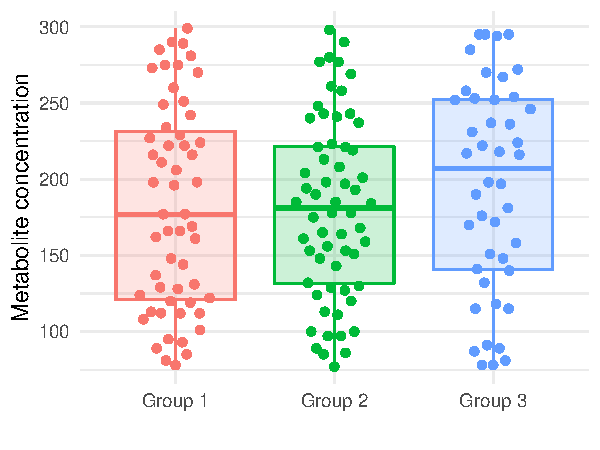
\includegraphics{computed_manuscript_files/figure-latex/plot-data-1.pdf}
\caption{\label{fig:plot-data}Metabolite concentration of clinical trial subjects}
\end{figure}

\hypertarget{code}{%
\section{Code}\label{code}}

The following code was used to load, merge, and plot the (simulated) clinical trial data:

\begin{Shaded}
\begin{Highlighting}[]
\CommentTok{\# load libraries}
\FunctionTok{library}\NormalTok{(tidyverse)}
\FunctionTok{library}\NormalTok{(ggbeeswarm)}
\FunctionTok{library}\NormalTok{(bookdown)}
\end{Highlighting}
\end{Shaded}

\begin{Shaded}
\begin{Highlighting}[]
\CommentTok{\# read in some initial data}
\NormalTok{df1 }\OtherTok{\textless{}{-}} \FunctionTok{read\_csv}\NormalTok{(}\StringTok{\textquotesingle{}data/example{-}data{-}1.csv\textquotesingle{}}\NormalTok{)}
\end{Highlighting}
\end{Shaded}

\begin{Shaded}
\begin{Highlighting}[]
\CommentTok{\# read new dataset}
\NormalTok{df2 }\OtherTok{\textless{}{-}} \FunctionTok{read\_csv}\NormalTok{(}\StringTok{\textquotesingle{}data/example{-}data{-}2.csv\textquotesingle{}}\NormalTok{)}
\end{Highlighting}
\end{Shaded}

\begin{Shaded}
\begin{Highlighting}[]
\CommentTok{\# merge datasets}
\NormalTok{final\_data }\OtherTok{\textless{}{-}} \FunctionTok{rbind}\NormalTok{(df1, df2)}
\end{Highlighting}
\end{Shaded}

\begin{Shaded}
\begin{Highlighting}[]
\CommentTok{\# plot the data}
\NormalTok{p }\OtherTok{\textless{}{-}}\NormalTok{ final\_data }\SpecialCharTok{\%\textgreater{}\%} 
  \FunctionTok{ggplot}\NormalTok{(}\FunctionTok{aes}\NormalTok{(}\AttributeTok{x =}\NormalTok{ class, }\AttributeTok{y =}\NormalTok{ conc, }\AttributeTok{color =}\NormalTok{ class)) }\SpecialCharTok{+}
  \FunctionTok{geom\_boxplot}\NormalTok{() }\SpecialCharTok{+}
\NormalTok{  ggbeeswarm}\SpecialCharTok{::}\FunctionTok{geom\_quasirandom}\NormalTok{(}\AttributeTok{width =} \FloatTok{0.25}\NormalTok{) }\SpecialCharTok{+} 
  \FunctionTok{xlab}\NormalTok{(}\StringTok{""}\NormalTok{) }\SpecialCharTok{+}
  \FunctionTok{ylab}\NormalTok{(}\StringTok{"Metabolite concentration"}\NormalTok{) }\SpecialCharTok{+} 
  \FunctionTok{theme\_minimal}\NormalTok{() }\SpecialCharTok{+}
  \FunctionTok{theme}\NormalTok{(}\AttributeTok{legend.position =} \StringTok{"none"}\NormalTok{)}
\NormalTok{p}
\end{Highlighting}
\end{Shaded}

\begin{table}

\caption{\label{tab:show-table-1}Initial subject data}
\centering
\begin{tabular}[t]{llrlllrlllr}
\toprule
ID & Class & Conc & | & ID & Class & Conc & | & ID & Class & Conc\\
\midrule
ID\_1 & Group 2 & 153 & | & ID\_34 & Group 2 & 221 & | & ID\_67 & Group 3 & 148\\
ID\_2 & Group 1 & 224 & | & ID\_35 & Group 1 & 112 & | & ID\_68 & Group 1 & 281\\
ID\_3 & Group 2 & 127 & | & ID\_36 & Group 3 & 246 & | & ID\_69 & Group 3 & 295\\
ID\_4 & Group 2 & 194 & | & ID\_37 & Group 2 & 190 & | & ID\_70 & Group 2 & 111\\
ID\_5 & Group 1 & 251 & | & ID\_38 & Group 1 & 177 & | & ID\_71 & Group 2 & 132\\
\addlinespace
ID\_6 & Group 1 & 81 & | & ID\_39 & Group 1 & 148 & | & ID\_72 & Group 2 & 261\\
ID\_7 & Group 2 & 100 & | & ID\_40 & Group 2 & 290 & | & ID\_73 & Group 1 & 122\\
ID\_8 & Group 1 & 270 & | & ID\_41 & Group 2 & 151 & | & ID\_74 & Group 2 & 124\\
ID\_9 & Group 2 & 100 & | & ID\_42 & Group 2 & 159 & | & ID\_75 & Group 1 & 234\\
ID\_10 & Group 1 & 161 & | & ID\_43 & Group 2 & 113 & | & ID\_76 & Group 2 & 184\\
\addlinespace
ID\_11 & Group 3 & 158 & | & ID\_44 & Group 1 & 249 & | & ID\_77 & Group 3 & 272\\
ID\_12 & Group 3 & 118 & | & ID\_45 & Group 1 & 124 & | & ID\_78 & Group 1 & 242\\
ID\_13 & Group 2 & 143 & | & ID\_46 & Group 3 & 87 & | & ID\_79 & Group 2 & 277\\
ID\_14 & Group 2 & 258 & | & ID\_47 & Group 1 & 166 & | & ID\_80 & Group 3 & 236\\
ID\_15 & Group 3 & 224 & | & ID\_48 & Group 1 & 196 & | & ID\_81 & Group 1 & 101\\
\addlinespace
ID\_16 & Group 3 & 254 & | & ID\_49 & Group 1 & 112 & | & ID\_82 & Group 3 & 218\\
ID\_17 & Group 3 & 190 & | & ID\_50 & Group 1 & 289 & | & ID\_83 & Group 2 & 130\\
ID\_18 & Group 2 & 148 & | & ID\_51 & Group 2 & 161 & | & ID\_84 & Group 1 & 128\\
ID\_19 & Group 1 & 89 & | & ID\_52 & Group 3 & 270 & | & ID\_85 & Group 3 & 252\\
ID\_20 & Group 2 & 89 & | & ID\_53 & Group 2 & 237 & | & ID\_86 & Group 1 & 198\\
\addlinespace
ID\_21 & Group 3 & 253 & | & ID\_54 & Group 2 & 280 & | & ID\_87 & Group 1 & 169\\
ID\_22 & Group 3 & 231 & | & ID\_55 & Group 2 & 175 & | & ID\_88 & Group 2 & 185\\
ID\_23 & Group 1 & 112 & | & ID\_56 & Group 2 & 223 & | & ID\_89 & Group 1 & 216\\
ID\_24 & Group 2 & 277 & | & ID\_57 & Group 3 & 295 & | & ID\_90 & Group 2 & 185\\
ID\_25 & Group 2 & 197 & | & ID\_58 & Group 1 & 275 & | & ID\_91 & Group 2 & 97\\
\addlinespace
ID\_26 & Group 2 & 208 & | & ID\_59 & Group 2 & 120 & | & ID\_92 & Group 2 & 165\\
ID\_27 & Group 2 & 193 & | & ID\_60 & Group 1 & 78 & | & ID\_93 & Group 3 & 89\\
ID\_28 & Group 3 & 141 & | & ID\_61 & Group 3 & 78 & | & ID\_94 & Group 2 & 221\\
ID\_29 & Group 1 & 206 & | & ID\_62 & Group 3 & 140 & | & ID\_95 & Group 1 & 162\\
ID\_30 & Group 2 & 168 & | & ID\_63 & Group 3 & 294 & | & ID\_96 & Group 1 & 131\\
\addlinespace
ID\_31 & Group 2 & 298 & | & ID\_64 & Group 3 & 295 & | & ID\_97 & Group 1 & 93\\
ID\_32 & Group 1 & 144 & | & ID\_65 & Group 3 & 285 & | & ID\_98 & Group 2 & 240\\
ID\_33 & Group 2 & 241 & | & ID\_66 & Group 2 & 129 & | & ID\_99 & Group 2 & 86\\
\bottomrule
\end{tabular}
\end{table}

\begin{table}

\caption{\label{tab:show-table-2}New subject data}
\centering
\begin{tabular}[t]{llrlllrlllr}
\toprule
ID & Class & Conc & | & ID & Class & Conc & | & ID & Class & Conc\\
\midrule
ID\_100 & Group 2 & 219 & | & ID\_120 & Group 2 & 85 & | & ID\_140 & Group 2 & 77\\
ID\_101 & Group 2 & 243 & | & ID\_121 & Group 3 & 181 & | & ID\_141 & Group 1 & 299\\
ID\_102 & Group 2 & 213 & | & ID\_122 & Group 3 & 216 & | & ID\_142 & Group 3 & 222\\
ID\_103 & Group 1 & 177 & | & ID\_123 & Group 1 & 222 & | & ID\_143 & Group 1 & 85\\
ID\_104 & Group 3 & 197 & | & ID\_124 & Group 3 & 252 & | & ID\_144 & Group 1 & 273\\
\addlinespace
ID\_105 & Group 2 & 198 & | & ID\_125 & Group 1 & 166 & | & ID\_145 & Group 3 & 115\\
ID\_106 & Group 1 & 120 & | & ID\_126 & Group 2 & 204 & | & ID\_146 & Group 1 & 290\\
ID\_107 & Group 3 & 170 & | & ID\_127 & Group 2 & 243 & | & ID\_147 & Group 2 & 269\\
ID\_108 & Group 3 & 78 & | & ID\_128 & Group 3 & 198 & | & ID\_148 & Group 2 & 97\\
ID\_109 & Group 1 & 129 & | & ID\_129 & Group 1 & 119 & | & ID\_149 & Group 1 & 229\\
\addlinespace
ID\_110 & Group 1 & 137 & | & ID\_130 & Group 1 & 198 & | & ID\_150 & Group 3 & 176\\
ID\_111 & Group 3 & 217 & | & ID\_131 & Group 3 & 151 & | & ID\_151 & Group 2 & 164\\
ID\_112 & Group 1 & 227 & | & ID\_132 & Group 3 & 115 & | & ID\_152 & Group 3 & 172\\
ID\_113 & Group 3 & 81 & | & ID\_133 & Group 3 & 237 & | & ID\_153 & Group 1 & 222\\
ID\_114 & Group 2 & 248 & | & ID\_134 & Group 2 & 178 & | & ID\_154 & Group 1 & 285\\
\addlinespace
ID\_115 & Group 1 & 211 & | & ID\_135 & Group 1 & 275 & | & ID\_155 & Group 2 & 153\\
ID\_116 & Group 1 & 113 & | & ID\_136 & Group 2 & 178 & | & ID\_156 & Group 3 & 132\\
ID\_117 & Group 1 & 216 & | & ID\_137 & Group 3 & 267 & | & ID\_157 & Group 2 & 156\\
ID\_118 & Group 3 & 91 & | & ID\_138 & Group 1 & 95 & | & ID\_158 & Group 1 & 260\\
ID\_119 & Group 3 & 258 & | & ID\_139 & Group 1 & 108 & | & ID\_159 & Group 2 & 201\\
\bottomrule
\end{tabular}
\end{table}

\hypertarget{colophon}{%
\section{Colophon}\label{colophon}}

This manuscript was built at \textbf{14 Jan 2022 15:10:08 MST} using the following computational environment and dependencies:

\begin{verbatim}
## R version 4.0.4 (2021-02-15)
## Platform: x86_64-apple-darwin17.0 (64-bit)
## Running under: macOS Mojave 10.14.6
## 
## Matrix products: default
## BLAS:   /Library/Frameworks/R.framework/Versions/4.0/Resources/lib/libRblas.dylib
## LAPACK: /Library/Frameworks/R.framework/Versions/4.0/Resources/lib/libRlapack.dylib
## 
## locale:
## [1] en_US.UTF-8/en_US.UTF-8/en_US.UTF-8/C/en_US.UTF-8/en_US.UTF-8
## 
## attached base packages:
## [1] stats     graphics  grDevices utils     datasets  methods   base     
## 
## other attached packages:
##  [1] bookdown_0.24    ggbeeswarm_0.6.0 forcats_0.5.1    stringr_1.4.0   
##  [5] dplyr_1.0.5      purrr_0.3.4      readr_2.1.1      tidyr_1.1.3     
##  [9] tibble_3.1.6     ggplot2_3.3.3    tidyverse_1.3.0 
## 
## loaded via a namespace (and not attached):
##  [1] Rcpp_1.0.7       lubridate_1.8.0  assertthat_0.2.1 digest_0.6.29   
##  [5] utf8_1.2.2       R6_2.5.1         cellranger_1.1.0 backports_1.2.1 
##  [9] reprex_2.0.0     evaluate_0.14    highr_0.9        httr_1.4.2      
## [13] pillar_1.6.4     rlang_0.4.12     readxl_1.3.1     rstudioapi_0.13 
## [17] rticles_0.22     rmarkdown_2.11   labeling_0.4.2   bit_4.0.4       
## [21] munsell_0.5.0    broom_0.7.6      compiler_4.0.4   vipor_0.4.5     
## [25] modelr_0.1.8     xfun_0.29        pkgconfig_2.0.3  htmltools_0.5.2 
## [29] tidyselect_1.1.1 fansi_1.0.0      crayon_1.4.2     tzdb_0.2.0      
## [33] dbplyr_2.1.0     withr_2.4.3      grid_4.0.4       jsonlite_1.7.2  
## [37] gtable_0.3.0     lifecycle_1.0.1  DBI_1.1.1        magrittr_2.0.1  
## [41] scales_1.1.1     cli_3.1.0        stringi_1.7.6    vroom_1.5.7     
## [45] farver_2.1.0     fs_1.5.2         xml2_1.3.3       ellipsis_0.3.2  
## [49] generics_0.1.1   vctrs_0.3.8      tools_4.0.4      bit64_4.0.5     
## [53] glue_1.6.0       beeswarm_0.4.0   hms_1.1.1        parallel_4.0.4  
## [57] fastmap_1.1.0    yaml_2.2.1       colorspace_2.0-0 rvest_1.0.2     
## [61] knitr_1.37       haven_2.3.1
\end{verbatim}

The current Git commit details are:

\begin{verbatim}
## [db20ac1] 2022-01-14: Merge branch 'main' of github.com:jperkel/computed_manuscript into main
\end{verbatim}

\hypertarget{references}{%
\section*{References}\label{references}}
\addcontentsline{toc}{section}{References}

\hypertarget{refs}{}
\begin{CSLReferences}{0}{0}
\leavevmode\hypertarget{ref-shen2014}{}%
\CSLLeftMargin{1. }
\CSLRightInline{Shen, H. Interactive notebooks: Sharing the code. \emph{Nature} \textbf{515}, 151--152 (2014).}

\leavevmode\hypertarget{ref-perkel2018a}{}%
\CSLLeftMargin{2. }
\CSLRightInline{Perkel, J. M. A toolkit for data transparency takes shape. \emph{Nature} \textbf{560}, 513--515 (2018).}

\leavevmode\hypertarget{ref-perkel2018}{}%
\CSLLeftMargin{3. }
\CSLRightInline{Perkel, J. M. Why Jupyter is data scientists{'} computational notebook of choice. \emph{Nature} \textbf{563}, 145--146 (2018).}

\leavevmode\hypertarget{ref-perkel2020}{}%
\CSLLeftMargin{4. }
\CSLRightInline{Perkel, J. M. Streamline your writing {{}} and collaborations {{}} with these reference managers. \emph{Nature} \textbf{585}, 149--150 (2020).}

\leavevmode\hypertarget{ref-perkel2021}{}%
\CSLLeftMargin{5. }
\CSLRightInline{Perkel, J. M. Reactive, reproducible, collaborative: computational notebooks evolve. \emph{Nature} \textbf{593}, 156--157 (2021).}

\end{CSLReferences}


\bibliographystyle{spbasic}
\bibliography{bibliography.bib}


\end{document}
